\documentclass{article}

\title{Dummit \& Foote Ch. 3.2: More on Cosets and Lagrange's Theorem}
\author{Scott Donaldson}
\date{Oct. 2023}
\usepackage{amsmath, amsthm, amsfonts, enumitem, tabu, tikz}

\begin{document}

\maketitle

Let $G$ be a group.

\section*{1. (10/1/23)}

Which of the following are permissible orders of subgroups of a group of order 120: 1, 2, 5, 7, 9, 15, 60, 240? For each permissible order give the corresponding index.

\begin{proof}
    From Lagrange's theorem, the order of a subgroup of a group of order 120 must divide 120. Then the permissible orders for subgroups are $1 = \frac{120}{120}$, $2 = \frac{120}{60}, 5 = \frac{120}{24}, 15 = \frac{120}{8}$, and $60 = \frac{120}{2}$. For each of these orders the index is given by the corresponding denumerator.
\end{proof}

\section*{2. (10/2/23)}

Prove that the lattice of subgroups of $S_3$ below is correct (i.e., prove that it contains all subgroups of $S_3$ and that their pairwise joins and intersections are correctly drawn).

\begin{center}
    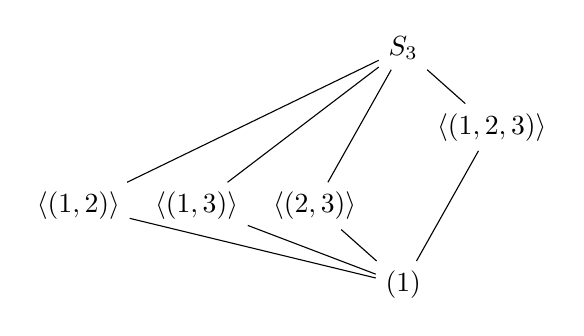
\begin{tikzpicture}[x=1.5cm]
        \node at (0, 0)          (1)  {$(1)$};
        \node at (-2.75, 1)      (12)  {$\langle (1, 2) \rangle$};
        \node at (-1.75, 1)      (13) {$\langle (1, 3) \rangle$};
        \node at (-0.75, 1)      (23) {$\langle (2, 3) \rangle$};
        \node at (0.75, 2)      (123) {$\langle (1, 2, 3) \rangle$};
        \node at (0, 3)       (S3)  {$S_3$};
        
        \draw (1) -- (12);
        \draw (1) -- (13);
        \draw (1) -- (23);
        \draw (1) -- (123);
        \draw (12) -- (S3);
        \draw (13) -- (S3);
        \draw (23) -- (S3);
        \draw (123) -- (S3);
    \end{tikzpicture}
\end{center}

\begin{proof}
    The symmetric group $S_3$ contains 6 elements. By Lagrange's theorem, its proper subgroups must have order 2 or 3. Each of the subgroups in the lattice above have order 2 or 3, so there are no smaller or larger subgroups not depicted above.

    From Corollary 10, a subgroup of order 2 must be isomorphic to $Z_2$, that is, cyclic and generated by a single element of order 2. The three subgroups generated by the three elements of order 2 (the 2-cycles of $S_3$) are depicted above. Similarly, a subgroup of order 3 must be isomorphic to $Z_3$ and generated by a single element of order 3. The subgroup generated by $(1, 2, 3)$ contains $(1, 3, 2)$, so there is only a single subgroup of order 3.

    Next, again by Lagrange's Theorem, a subgroup of two different containing groups must have an order that divides the order of both of the containing groups. First consider a subgroup of order 2 and a subgroup of order 3. Only 1 divides 2 and 3, so the intersection must be the identity. Similarly, if a subgroup of order 2 and a subgroup of order 3 are contained in a larger group, then that group's order must have both 2 and 3 as divisors. The smallest integer for which this is possible is 6, which is the order of all of $S_3$.

    Finally, consider a pair of subgroups of order 2. Their intersection is either the identity or else they are the same subgroup. Their join must have even order, but 4 does not divide 6 and any larger even number exceeds the order of $S_3$. Thus their join is all of $S_3$. This concludes the proof that the lattice of subgroups of $S_3$ is correct.
\end{proof}

\end{document}